
\documentclass{beamer}

\usepackage{algpseudocode, color, colortbl, listings, MnSymbol}

\usepackage{hyperref}
\hypersetup{
    colorlinks=true,
    urlcolor=blue,
}

\usetheme{Montpellier}
\usecolortheme{rose}

% page numbers, from
% https://tex.stackexchange.com/questions/137022/how-to-insert-page-number-in-beamer-navigation-symbols
\expandafter\def\expandafter\insertshorttitle\expandafter{%
  \insertshorttitle\hfill%
  \insertframenumber\,/\,\inserttotalframenumber}

\definecolor{Gray}{gray}{0.8}
\newcolumntype{g}{>{\columncolor{Gray}}c}

\newcommand{\stanza}{ \\~\ }

\title{19. Dynamic Programming}
\subtitle{CPSC 535}
\author{Kevin A. Wortman}
\institute{ 
\includegraphics[height=2cm]{csuf-logo-cmyk} }
\date{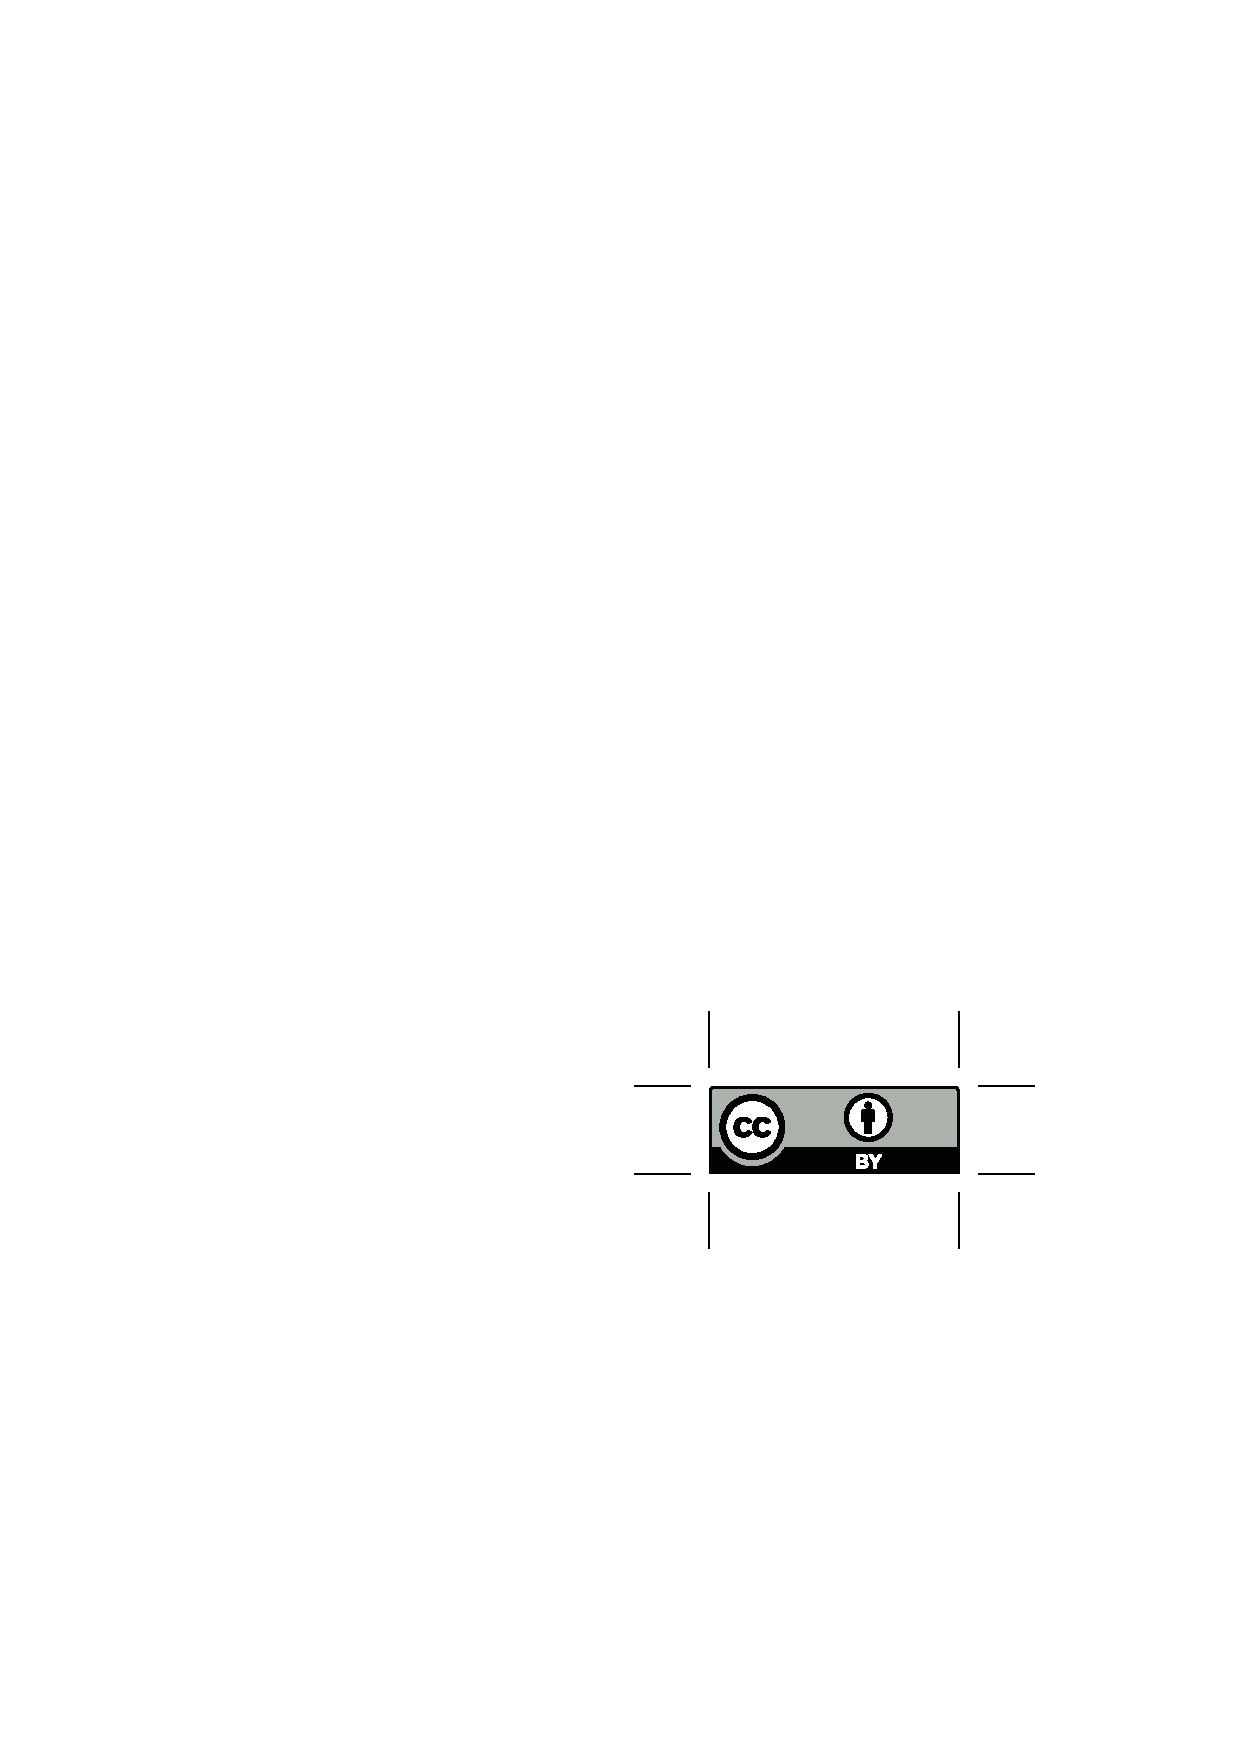
\includegraphics[height=14pt]{by} \\

{\tiny
This work is licensed under a
\href{http://creativecommons.org/licenses/by/4.0/}{Creative Commons Attribution 4.0 International License}.
}}

\begin{document}

\begin{frame}
  \titlepage
\end{frame}

\begin{frame} \frametitle{Dynamic Programming}
  \begin{itemize}
  \item \textbf{Dynamic programming:} pattern for solving problems with a divide-and-conquer structure \emph{and overlapping subproblems}
  \item Note: ``programming'' does not refer to coding
  \item Similar to divide-and-conquer
    \begin{itemize}
    \item Recall: merge sort, closest pair
    \end{itemize}
  \item Only applies to a narrow category of problems
  \item \textbf{But} offers huge speed-ups in those rare cases
    \begin{itemize}
    \item often exponential $\longrightarrow$ fast polynomial
    \end{itemize}
  \end{itemize}
\end{frame}

\begin{frame} \frametitle{Designing Dynamic Programming Algorithms}
Suggested process to design a dynamic programming algorithm:
  \begin{enumerate}
  \item Characterize the structure of an optimal solution (i.e. data type)
  \item Recursively define the value of an optimal solution (like divide-and-conquer)
  \item Design pseudocode that computes the \textbf{value} of an optimal solution
    \begin{itemize}
    \item Either \emph{bottom-up,} or with \emph{memoization}
    \end{itemize}
  \item (If desired, next class) Design pseudocode that constructs an optimal solution based on information computed in step 3.
  \end{enumerate}
\end{frame}

\begin{frame} \frametitle{Rod Cutting Problem}

  \emph{rod cutting problem} \\
  \textbf{input:} integer rod length $n \geq 0$ and a table of prices $p_1, \ldots, p_n$ \\
  \textbf{output:} maximum revenue obtainable by cutting the rod into pieces of length $\leq n$ \stanza

  (Above computes a \emph{value} of a solution, to compute an actual
  \emph{solution} change the \textbf{output} to:)
  \stanza

  \textbf{output:} a list of rod-lengths in $[1, n]$ that add up to exactly $n$ and maximize revenue

\end{frame}

\begin{frame} \frametitle{Greedy Doesn't Work}

  \begin{itemize}
  \item Tempting to try a greedy heuristic
    \begin{itemize}
    \item e.g. pick the length with the best unit price $p_i/i$
    \end{itemize}
  \item \textbf{But} greedy algorithms for this problem are \textbf{not correct}
  \item Problem definition makes \textbf{no guarantee} that
    \begin{itemize}
    \item prices $p_i$ obey common-sense properties
    \item e.g. larger pieces are more valuable than smaller ones
    \item e.g. buying in bulk is a better deal
    \item e.g. small scraps like $p_1$ are nearly worthless
    \end{itemize}
  \item In general, problems that benefit from dynamic programming cannot be solved correctly by greedy methods
  \item If you design a greedy alg., onus is on you to prove correctness
  \item \emph{Tip:} if a problem is framed as dynamic programming, don't even bother with greedy approaches
  \end{itemize}
\end{frame}

\begin{frame} \frametitle{Baseline: Exhaustive Search}
  \begin{itemize}
  \item Baseline idea: try every way of dividing length $n$ into smaller pieces
  \item $\approx 2^n$ candidates
  \item $O(2^n)$ time
  \item extremely slow
  \end{itemize}
\end{frame}

\begin{frame} \frametitle{1. Characterize Solution}
  \begin{itemize}
  \item recall: $p_i = $ price of a rod of length $i$
  \item a solution is a sequence of rod-lengths $S = \langle i_1, i_2, \ldots, i_k \rangle$ such that $\sum_j i_j = n$ and the total revenue
    \[ \sum_j p_{i_j} \]
    is maximized
  \item define
    \[ r_i = \text{ the \textbf{maximum revenue obtainable} from a rod of length } i \]
  \item the \textbf{optimal value} is $r_n$
  \end{itemize}
\end{frame}
    
\begin{frame} \frametitle{2. Recursive Definition of an Optimal Solution}
  \begin{itemize}
  \item Each piece must have length $\geq 1,$ so each $i_j \in [1, n]$
  \item Given original length $n$, we could make one cut to form: \\
    $1+(n-1), 2+(n-2), 3+(n-3), \ldots, n+0$ \\
    (last entry means to keep the rod whole; no cut)
  \item These produce revenue
    $p_1+r_{n-1}, p_2 +r_{n-2}, p_3+r_{n-3}, \ldots, p_n + r_0$
  \item Goal is to \textbf{maximize} revenue
  \item So $r_n = \max(p_1+r_{n-1}, p_2 +r_{n-2}, p_3+r_{n-3}, \ldots, p_n + r_0)$ i.e.
    \[ r_n = \max_{1 \leq i \leq n} (p_i + r_{n-i}) \]
  \end{itemize}
  \end{frame}

\begin{frame} \frametitle{Aside: Recursive Top-Down Algorithm}
  {\small
    \begin{algorithmic}[1]
      \Function{CUT-ROD}{$p[0..n], n$}
      \If { $n=0$ }
        \State \Return 0
      \EndIf
      \State $q = -\infty$
      \For { $i=1$ to $n$ }
        \State $q = \max(q, p[i] + \text{CUT-ROD}(p, n-i))$
      \EndFor
      \State \Return $q$
    \EndFunction
    \end{algorithmic}
  }
  \vspace{.5cm}

    \textbf{Overlapping subproblems:} ex. CUT-ROD($p, 2$) will be computed many times \\
    \textbf{Slow;} $O(2^n)$ time
\end{frame}

\begin{frame} \frametitle{Enter Dynamic Programming}
  \begin{itemize}
  \item Problem: top-down recursion recomputes the same values over and over
  \item Solution: use a \textbf{table} (array) to cache these solutions
  \item For each $x$, evaluate
    \[ \text{CUT-ROD}(p, x) \]
    \textbf{only once}
  \item Time/space trade-off
    \begin{itemize}
    \item table takes extra space
    \item saves a \textbf{lot} of time
    \item exponential $\longrightarrow$ polynomial
    \end{itemize}
  \end{itemize}
\end{frame}

\begin{frame} \frametitle{Memoization and Bottom-Up}
  \begin{itemize}
  \item Two fine approaches for caching subsolutions
  \item \textbf{Memoization:} use an array or hash table $T$, where
    \begin{center}
      $T[i]$ = solution for input $i$, or dummy value if undefined
    \end{center}
  \item CUT-ROD is still recursive, but has a base case to reuse $T[i]$ instead of evaluating the function body
  \item \textbf{Bottom-Up:} solve subproblems from smallest to largest
  \item Initialize $T[0], T[1], \ldots, T[n]$ in an interative loop
  \item Mostly a matter of preference
  \item Some programming languages support automatic memoization (ex. Racket)
  \end{itemize}
  \end{frame}

\begin{frame} \frametitle{3. Pseudocode for \textbf{Memoized} Dynamic Programming Alg.}
      {\footnotesize
      \begin{algorithmic}[1]
        \Function{MEMOIZED-CUT-ROD}{$p[0..n], n$}
        \State Create empty hash map $H$
        \State \Return CUT-ROD-REC($p, n, H$)
        \EndFunction
      \Function{CUT-ROD-REC}{$p[0..n], n, H$}
        \If{ H.CONTAINS-KEY($n$) }
        \State \Return $H[n]$
        \EndIf
      \If { $n=0$ }
        \State \Return 0
      \EndIf
      \State $q = -\infty$
      \For { $i=1$ to $n$ }
        \State $q = \max(q, p[i] + \text{CUT-ROD-REC}(p, n-i, H))$
        \EndFor
        \State $H[n] = q$
      \State \Return $q$
    \EndFunction
      \end{algorithmic}
      }
\end{frame}

\begin{frame} \frametitle{3. Pseudocode for \textbf{Bottom-Up} Dyn. Prog. Alg.}
  \begin{algorithmic}[1]
    \Function{BOTTOM-UP-CUT-ROD}{$p[0..n], n$}
    \State Create new array $r[0..n]$
    \State $r[0] = 0$ \Comment{ base case }
    \For { $j = 1 $ to $n$ } \Comment{general cases bottom-up}
      \State $q = -\infty$
      \For { $i = 1 $ to $j$ }
      \Comment{only references initialized elements}
        \State $q = \max(q, p[i] + r[j-1])$ 
      \EndFor
      \State $r[j] = q$
      \EndFor
      \State \Return $r[n]$
      \EndFunction
  \end{algorithmic}
  \end{frame}

\begin{frame} \frametitle{Analysis}
  \begin{itemize}
  \item BOTTOM-UP-CUT-ROD: clearly $\Theta(n^2)$ b/c nested for loops
  \item MEMOIZED-CUT-ROD:
    \begin{itemize}
    \item Less clear, but $\Theta(n^2)$ expected time
    \item Cache hit ($H$ contains $n$): $\Theta(1)$ expected time
    \item Cache miss: $\Theta(n)$ expected time due to for loop
    \item Observe: each miss happens \emph{at most once}
    \item Total time at most
      \[ \sum_{i=0}^n \Theta(i) \in \Theta(n^2) \]
    \end{itemize}
  \item Same $\Theta(n^2)$ efficiency; memoized version is expected
  \item \textbf{Huge} speedup: $O(2^n) \longrightarrow \Theta(n^2)$
  \item Modest $\Theta(n)$ space complexity for table
  \end{itemize}
\end{frame}

\begin{frame} \frametitle{What's Next}
  \begin{itemize}
  \item Computing a solution (list of rod-lengths)
  \item Maximizing over two indices
  \item Longest common subsequence problem
  \end{itemize}
\end{frame}

\end{document}
